\documentclass[border=12pt]{standalone}
\usepackage{tikz}
\usetikzlibrary{shapes.geometric, arrows.meta, positioning, calc, fit, backgrounds}
\usepackage{fontspec}
\setmainfont{DejaVu Sans}

\begin{document}
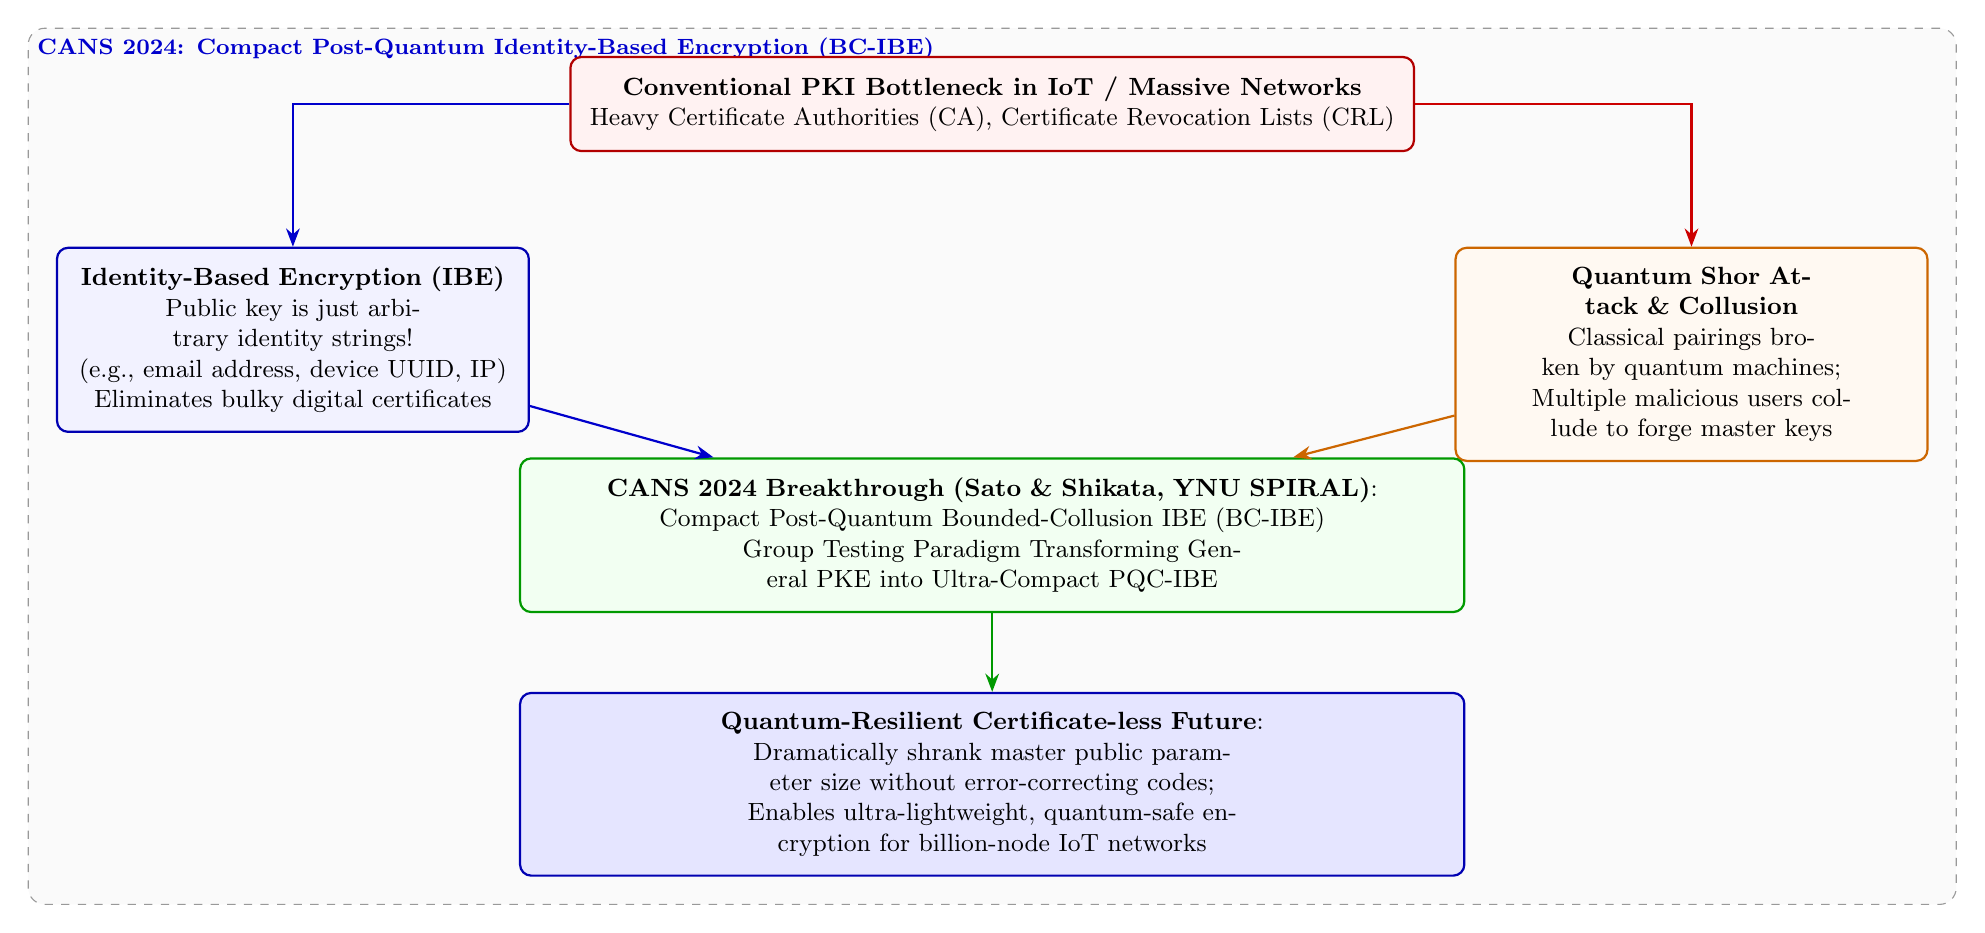
\begin{tikzpicture}[
    font=\small,
    >=Stealth,
    node distance=1.2cm,
    block/.style={rectangle, draw=blue!70!black, fill=blue!5, rounded corners=4pt, thick, align=center, inner sep=7pt},
    alertblock/.style={rectangle, draw=red!70!black, fill=red!5, rounded corners=4pt, thick, align=center, inner sep=7pt},
    greenblock/.style={rectangle, draw=green!60!black, fill=green!5, rounded corners=4pt, thick, align=center, inner sep=7pt},
    amberblock/.style={rectangle, draw=orange!80!black, fill=orange!5, rounded corners=4pt, thick, align=center, inner sep=7pt},
    groupbox/.style={draw=black!40, dashed, rounded corners=6pt, fill=black!2, inner sep=10pt}
]

    % Top Problem: Public-Key Distribution Bottleneck
    \node[alertblock] (pki) {\textbf{Conventional PKI Bottleneck in IoT / Massive Networks}\\Heavy Certificate Authorities (CA), Certificate Revocation Lists (CRL)};

    % Identity-Based Encryption Promise
    \node[block, below left=1.2cm and 0.5cm of pki, text width=5.5cm] (ibe) {\textbf{Identity-Based Encryption (IBE)}\\Public key is just arbitrary identity strings!\\(e.g., email address, device UUID, IP)\\Eliminates bulky digital certificates};

    % Quantum Threat & Collusion Risk
    \node[amberblock, below right=1.2cm and 0.5cm of pki, text width=5.5cm] (quantum) {\textbf{Quantum Shor Attack \& Collusion}\\Classical pairings broken by quantum machines;\\Multiple malicious users collude to forge master keys};

    \draw[->, thick, blue!80!black] (pki) -| (ibe);
    \draw[->, thick, red!80!black] (pki) -| (quantum);

    % Central Breakthrough: CANS 2024
    \node[greenblock, below=1.4cm of $(ibe)!0.5!(quantum)$, text width=11.5cm] (cans) {\textbf{CANS 2024 Breakthrough (Sato \& Shikata, YNU SPIRAL)}:\\Compact Post-Quantum Bounded-Collusion IBE (BC-IBE)\\Group Testing Paradigm Transforming General PKE into Ultra-Compact PQC-IBE};

    \draw[->, thick, blue!80!black] (ibe) -- (cans);
    \draw[->, thick, orange!80!black] (quantum) -- (cans);

    % Bottom Result
    \node[block, fill=blue!10, below=1.0cm of cans, text width=11.5cm] (impact) {\textbf{Quantum-Resilient Certificate-less Future}:\\Dramatically shrank master public parameter size without error-correcting codes;\\Enables ultra-lightweight, quantum-safe encryption for billion-node IoT networks};
    \draw[->, thick, green!60!black] (cans) -- (impact);

    \begin{scope}[on background layer]
        \node[groupbox, fit=(pki) (ibe) (quantum) (cans) (impact), label={[anchor=north west, font=\footnotesize\bfseries, blue!80!black]north west:CANS 2024: Compact Post-Quantum Identity-Based Encryption (BC-IBE)}] {};
    \end{scope}

\end{tikzpicture}
\end{document}
